%!/usr/bin/env pdflatex
%-*- coding: utf-8 -*-
%@author : Romain Graux
%@date : 2022 Mar 08, 16:20:03
%@last modified : 2022 Mar 16, 13:45:11


% [ PLAN ] 
% - Motivation
%   - Classical compressors (JPEG, ...)
%   - What we need (tasks)
%   - What they built
% - Intuition
%   - Example on MNIST

\documentclass[10pt,t]{beamer}


% Import all packages
\usepackage{graphicx,xcolor,caption}

% Color declarations
\definecolor{greyBackgroundColor}{rgb}{0.8,0.8,0.8}
\definecolor{primaryColor}{rgb}{0.5,0,0.5}
\definecolor{secondaryColor}{rgb}{0,0,0}

% Theme definition and progessbar settings
\usetheme[progressbar=frametitle]{metropolis}
\useinnertheme{metropolis}
\useoutertheme{metropolis}
\setbeamertemplate{frame numbering}[fraction]
\setbeamertemplate{navigation symbols}{
      \vbox{
          \hbox{\insertslidenavigationsymbol}
          \hbox{\insertframenavigationsymbol}
          \hbox{\insertbackfindforwardnavigationsymbol}
          \vfill
      }
}
% \setbeamercovered{transparent}

% Settings of all colors
\setbeamercolor{background canvas}{bg=white}
\setbeamercolor{title}{fg=primaryColor}
\setbeamercolor{frametitle}{bg=greyBackgroundColor, fg=primaryColor}
\setbeamercolor{structure}{fg=primaryColor}
\setbeamercolor{subsection in head/foot}{fg=secondaryColor}
\setbeamercolor{progress bar}{fg=primaryColor}

% Personal commands declaration
% Symbols
\newcommand{\Tau}{\mathcal{T}}
% all path commands
\newcommand{\docsPath}[1]{./docs/#1}
\newcommand{\imgsPath}[1]{\docsPath{imgs/#1}}
\newcommand{\mnistPath}[1]{\imgsPath{mnist/#1}}
% visualization commands
\newcommand{\question}[1]{\colorbox{primaryColor!15}{\large{\color{secondaryColor}#1}}}
\newcommand{\keyPoint}[1]{\color{secondaryColor}{\textbf{#1}}}
\newcommand{\alignCovered}[1]{%
        \setbeamercovered{transparent}
        \begin{align*}
            #1
        \end{align*}
}

% Meta information declaration
\title{Lossy compression for lossless prediction}
\subtitle{EECS Seminar: Advanced Topics in Machine Learning}
\author{Romain Graux}
\date{\today}

\begin{document}
\metroset{block=fill}

\begin{frame}
    \titlepage
\end{frame}

\begin{frame}{Motivation}
    $\sim50$ trillion GB data collected per year

    \only<2->{
        $\Rightarrow$ But most data is processed by algorithms performing \textbf{downstream tasks}.
    \vspace{5pt}
    }

    \def \imgWidth {0.23\textwidth}
    

    \only<3>{
        \begin{figure}
            \centering
            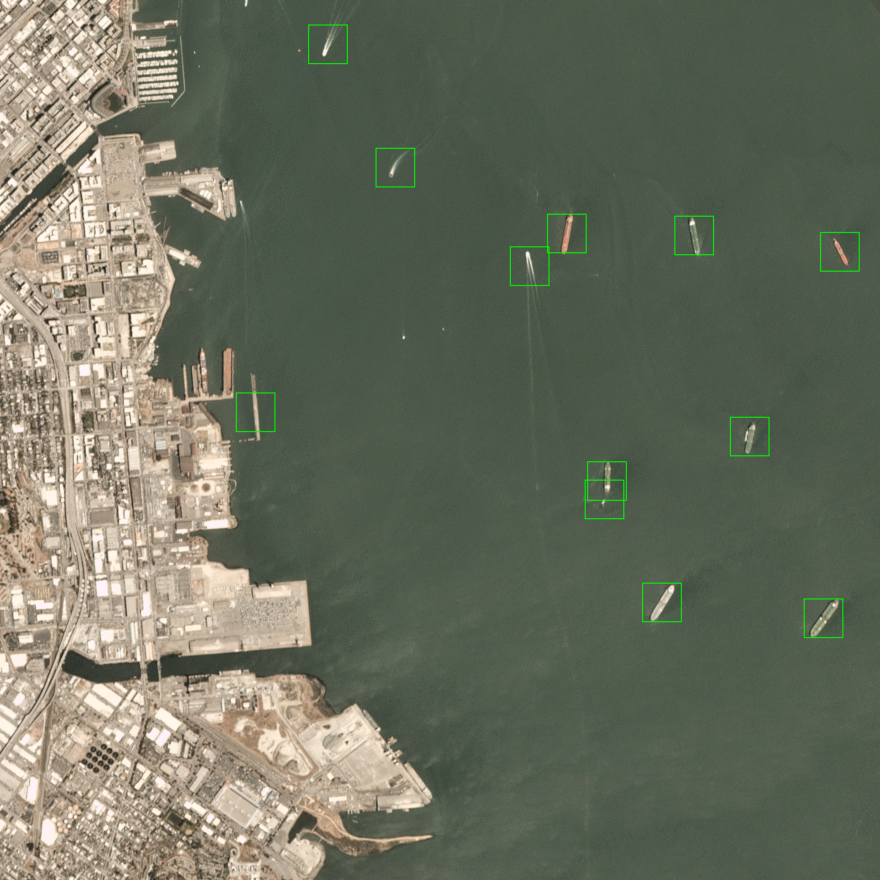
\includegraphics[width=\imgWidth]{\imgsPath{applications/satellite-detection.png}} \quad
            \includegraphics[width=\imgWidth]{\imgsPath{void.png}} \\
            \includegraphics[width=\imgWidth]{\imgsPath{void.png}} \quad
            \includegraphics[width=\imgWidth]{\imgsPath{void.png}} 
        \end{figure}
    }

    \only<4>{
        \begin{figure}
            \centering
            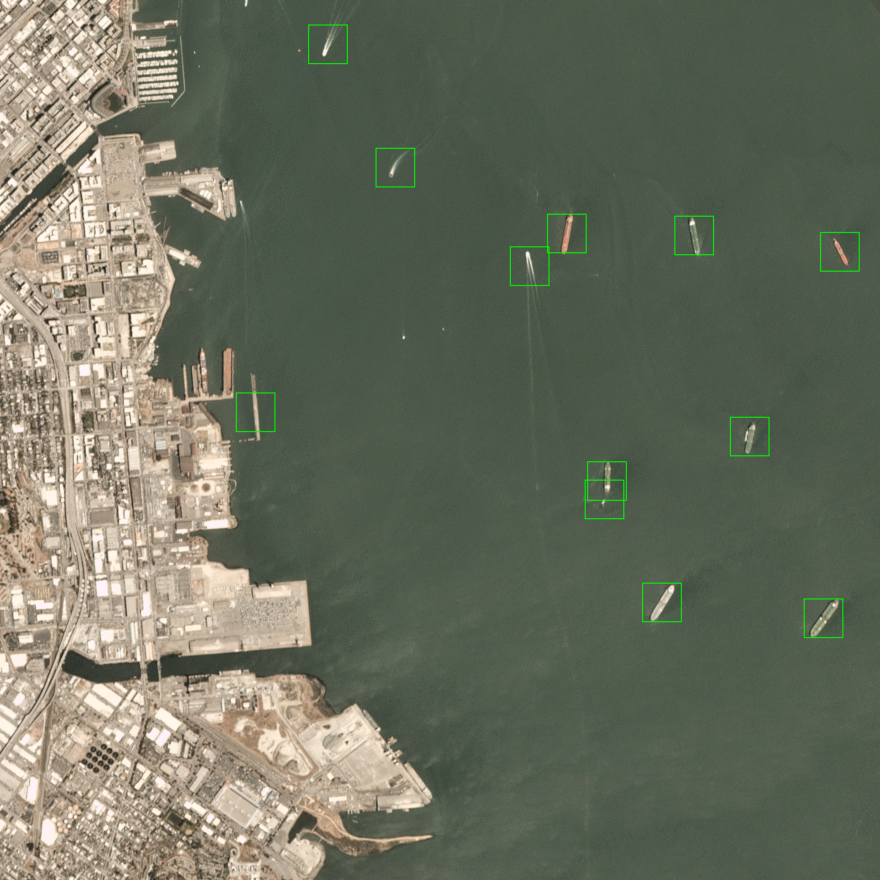
\includegraphics[width=\imgWidth]{\imgsPath{applications/satellite-detection.png}} \quad
            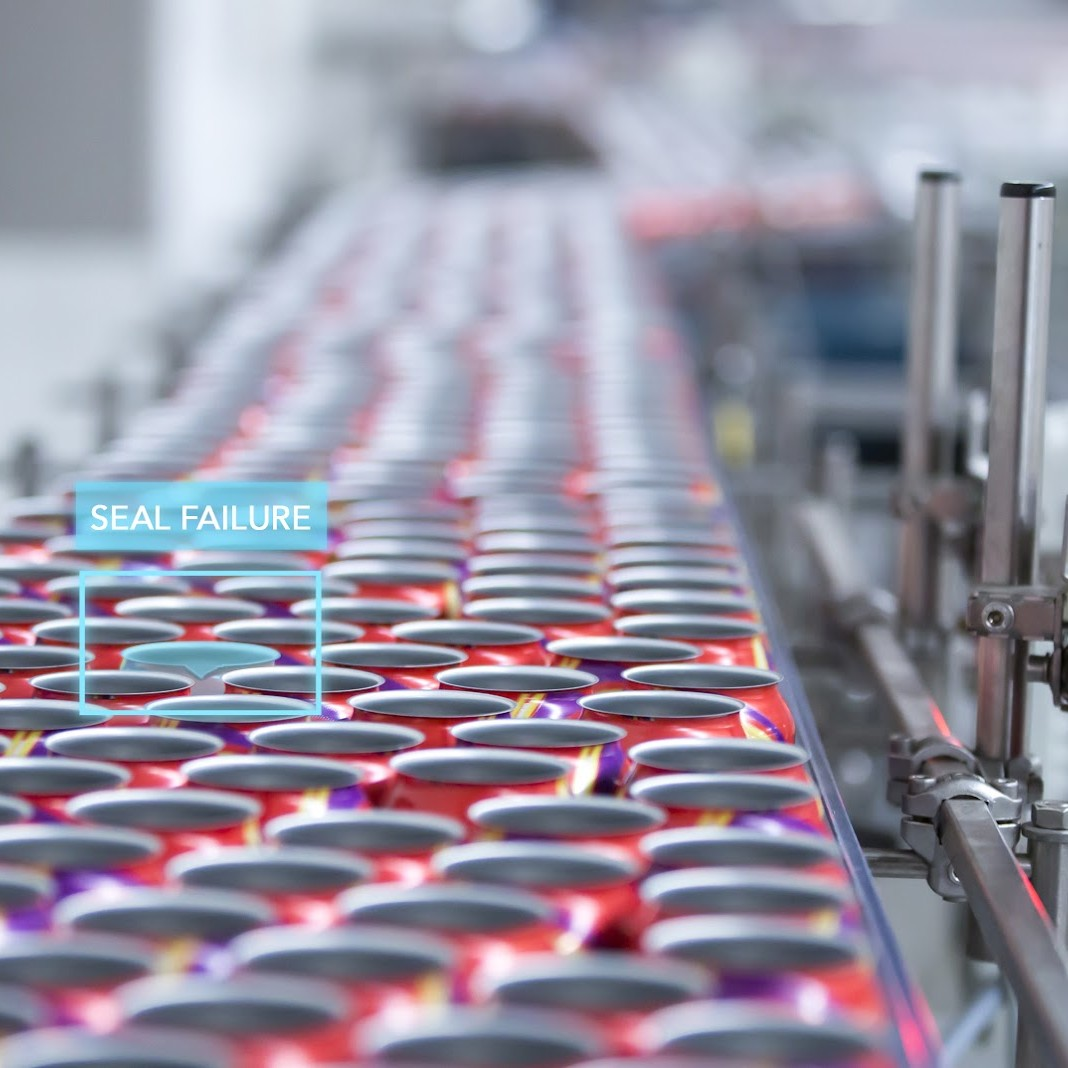
\includegraphics[width=\imgWidth]{\imgsPath{applications/quality_control.jpg}} \\
            \includegraphics[width=\imgWidth]{\imgsPath{void.png}} \quad
            \includegraphics[width=\imgWidth]{\imgsPath{void.png}} 
        \end{figure}
    }

    \only<5>{
        \begin{figure}
            \centering
            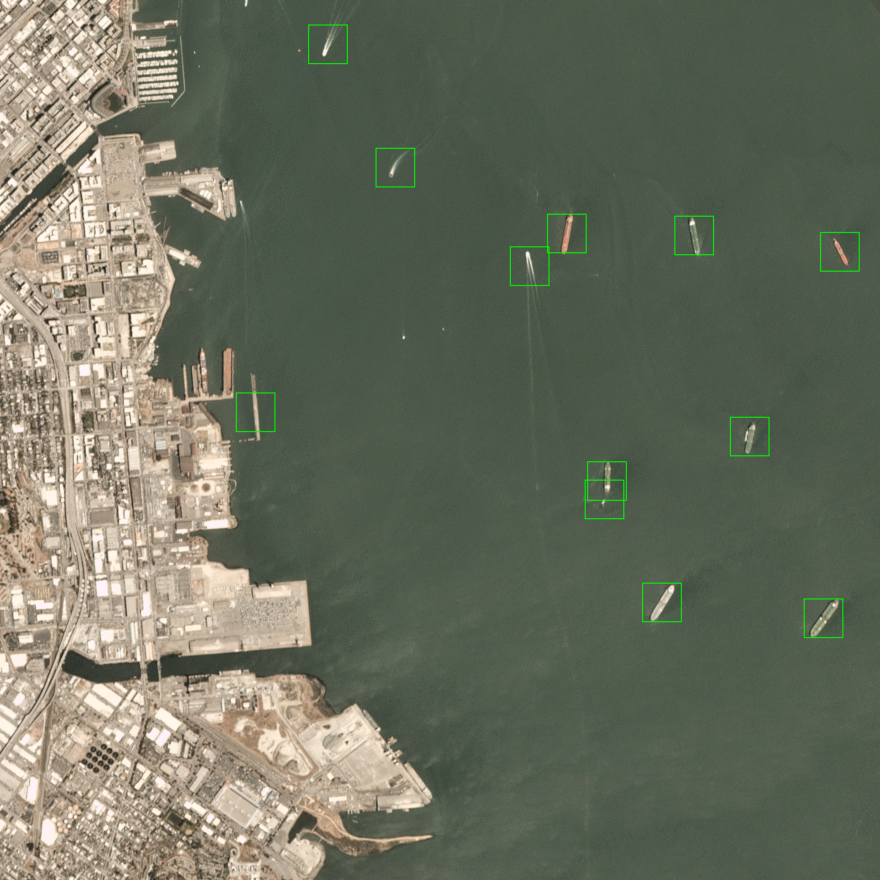
\includegraphics[width=\imgWidth]{\imgsPath{applications/satellite-detection.png}} \quad
            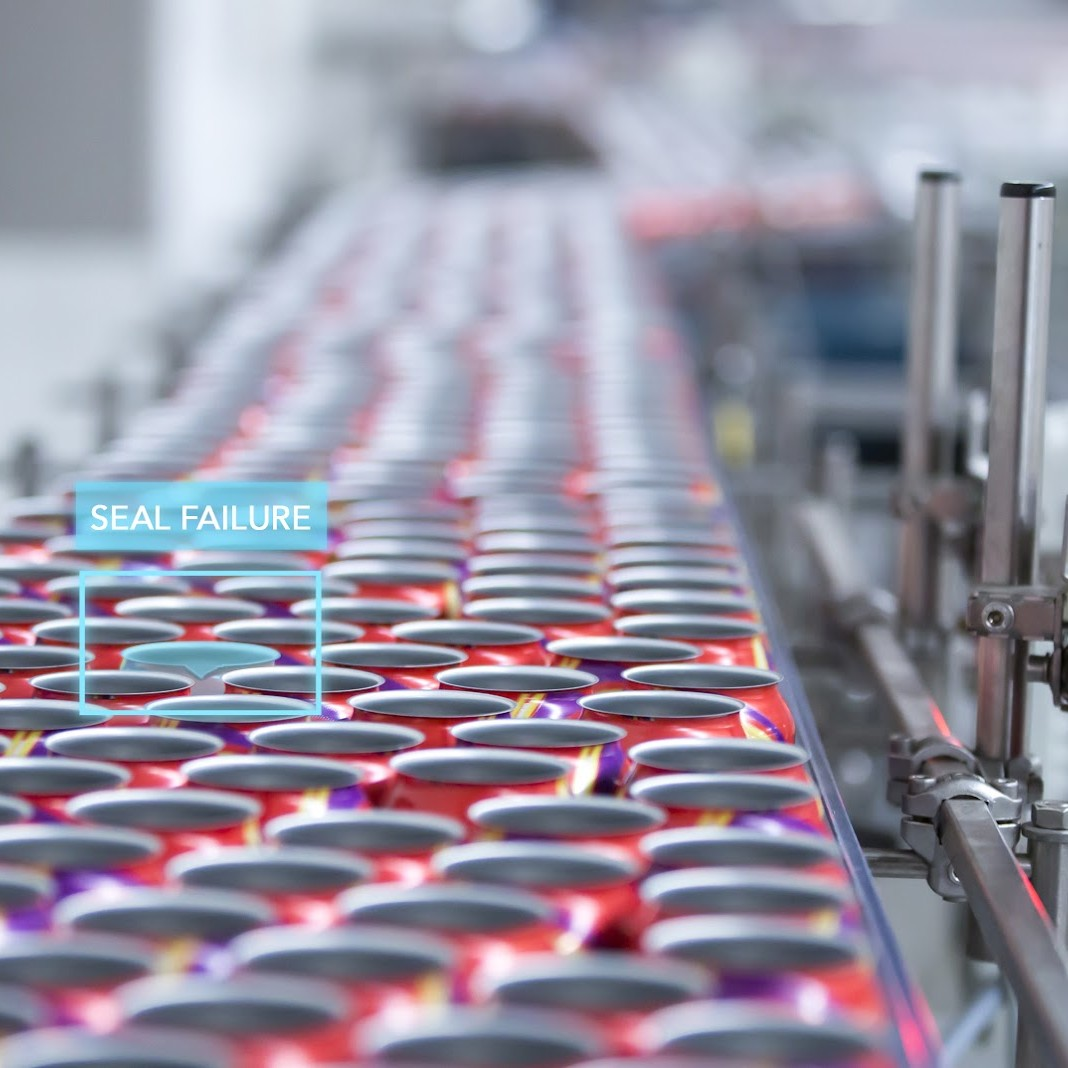
\includegraphics[width=\imgWidth]{\imgsPath{applications/quality_control.jpg}} \\[12pt]
            \includegraphics[width=\imgWidth]{\imgsPath{void.png}} \quad
            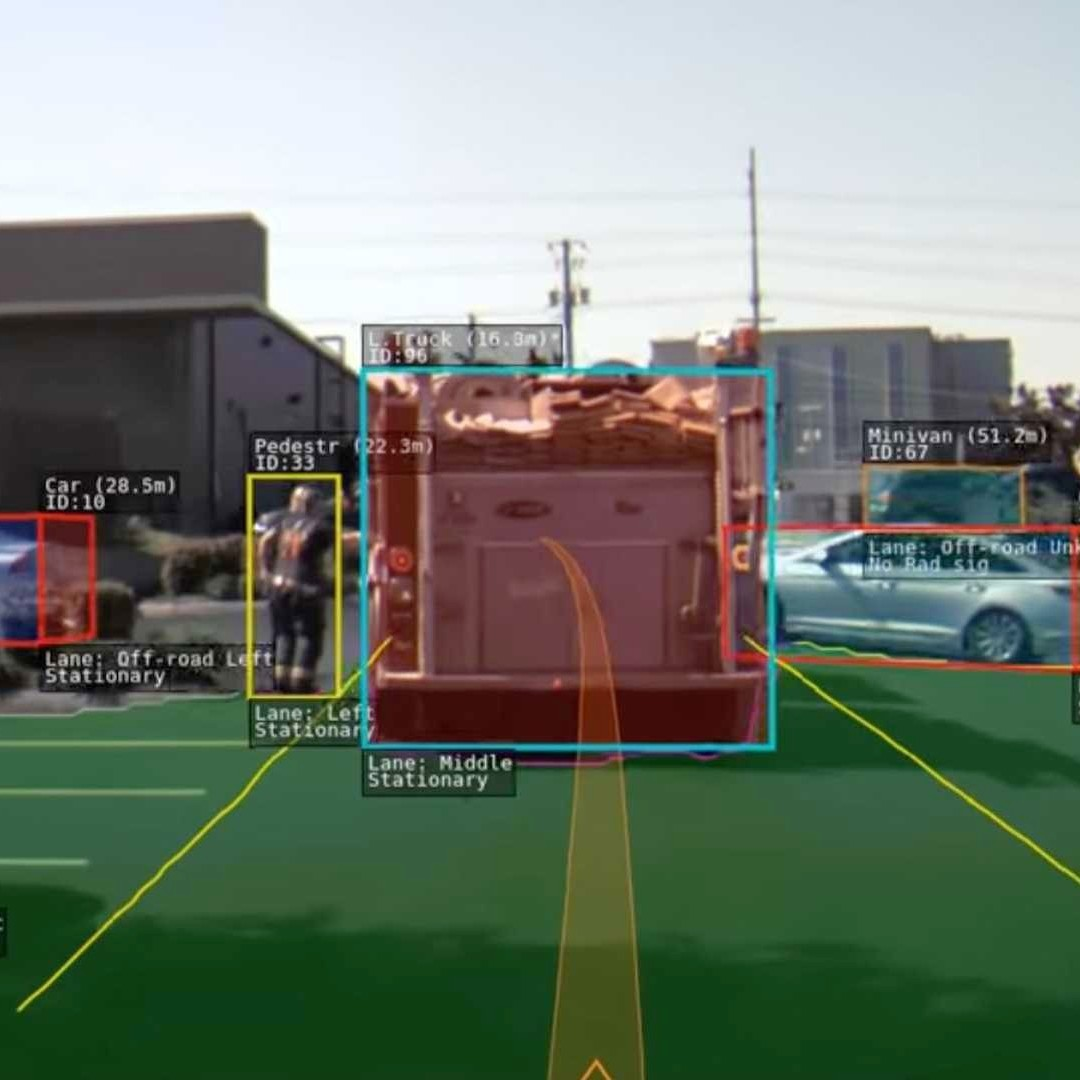
\includegraphics[width=\imgWidth]{\imgsPath{applications/selfdriving-cars.jpeg}} 
        \end{figure}
    }

    \only<6>{
        \begin{figure}
            \centering
            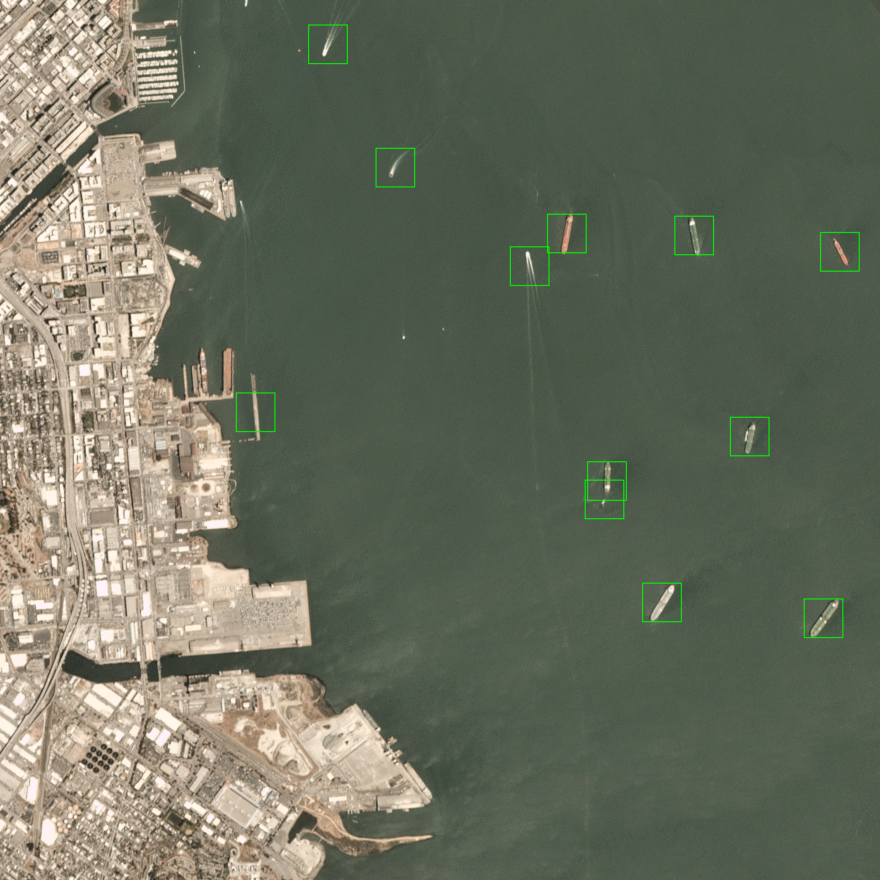
\includegraphics[width=\imgWidth]{\imgsPath{applications/satellite-detection.png}} \quad
            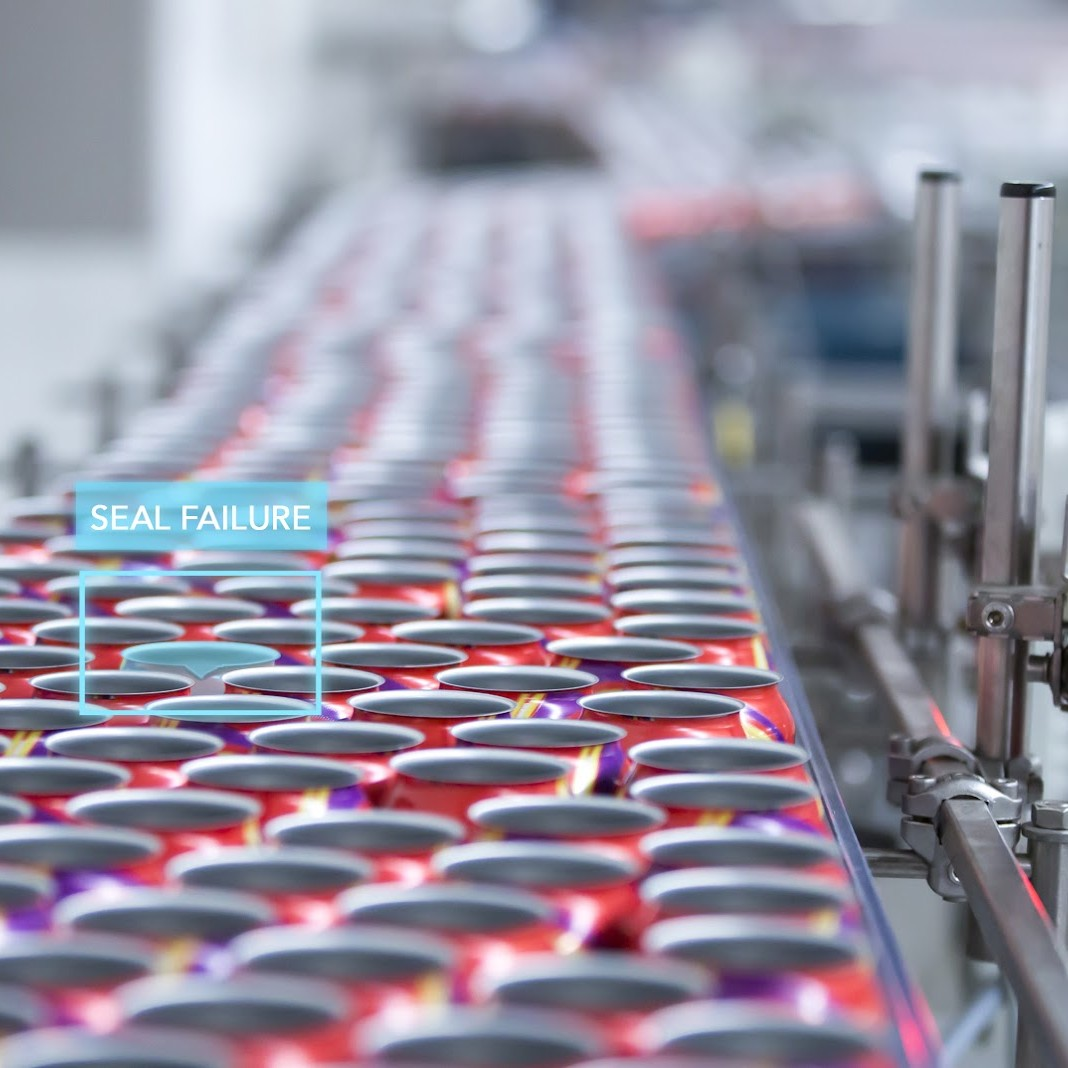
\includegraphics[width=\imgWidth]{\imgsPath{applications/quality_control.jpg}} \\[12pt]
            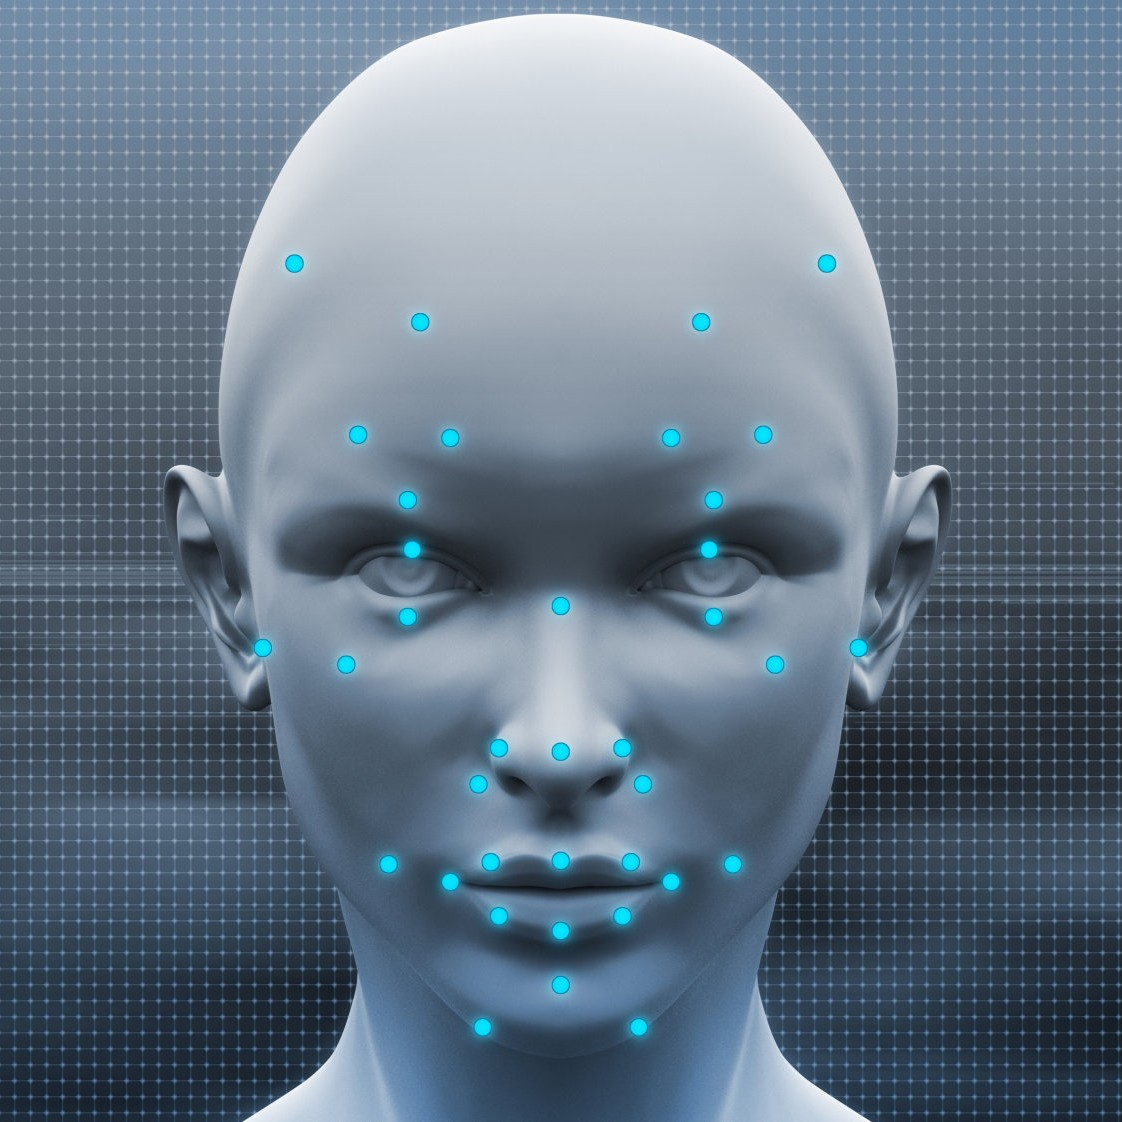
\includegraphics[width=\imgWidth]{\imgsPath{applications/face-recognition.jpeg}} \quad
            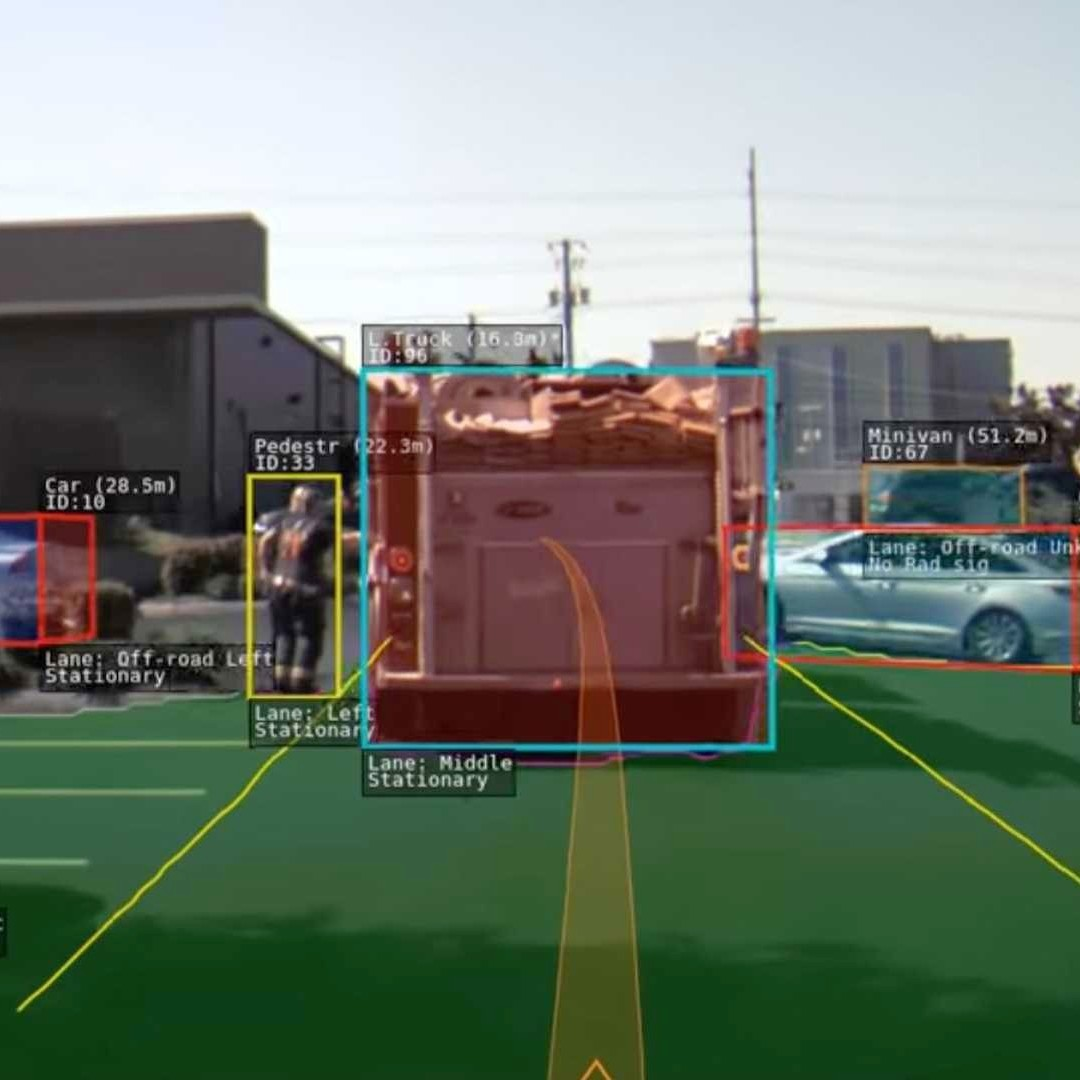
\includegraphics[width=\imgWidth]{\imgsPath{applications/selfdriving-cars.jpeg}} 
        \end{figure}
    }

    \only<7->{
        Yet current compressors optimize high \textbf{perceptual} fidelity
    }

    \only<8->{
        \begin{itemize}
            \item Stores too much not needed information
            \item Does not ensure good task performance
        \end{itemize}
    }


    \vfill
    \begin{columns}
    \column{0.2\textwidth}
    \only<9->{
            \begin{figure}
                \centering
                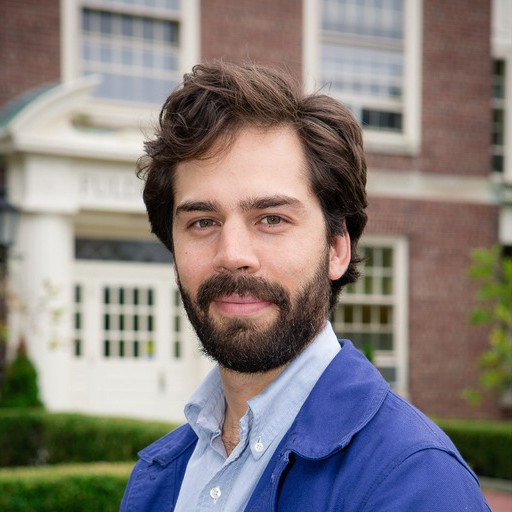
\includegraphics[width=\textwidth]{\imgsPath{chris/source.jpeg}}
                \caption*{Source}
                \label{fig:chris-source}
            \end{figure}
    }

    \column{0.2\textwidth}
    \only<10->{
            \begin{figure}
                \centering
                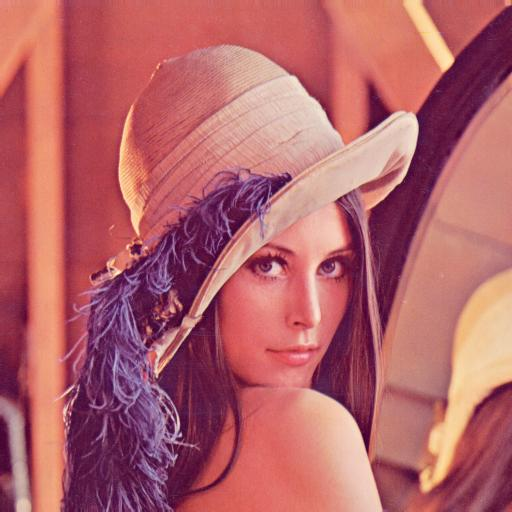
\includegraphics[width=\textwidth]{\imgsPath{chris/high.jpeg}}
                \caption*{High bitrate}
                \label{fig:chris-high}
            \end{figure}
    }

    \column{0.2\textwidth}
    \only<11->{
            \begin{figure}
                \centering
                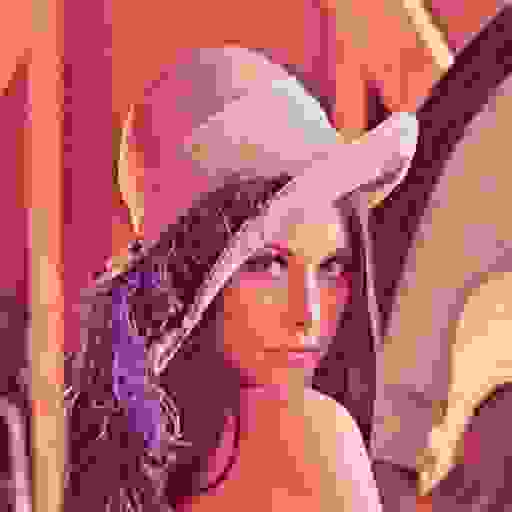
\includegraphics[width=\textwidth]{\imgsPath{chris/low.jpeg}}
                \caption*{Low bitrate}
                \label{fig:chris-low}
            \end{figure}
    }

    \column{0.2\textwidth}
    \only<12->{
            \begin{figure}
                \centering
                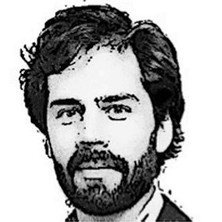
\includegraphics[width=\textwidth]{\imgsPath{chris/desired.jpeg}}
                \caption*{Desired}
                \label{fig:chris-desired}
            \end{figure}
    }
    \end{columns}
\end{frame}

\begin{frame}{What they designed}
    \begin{center}
        \large{They designed a \textbf{task-centric} distortion that ensures good downstream performance}
    \end{center}
    \pause
    \vfill
    \begin{itemize}[<+->]
        \item Characterize minimum bit-rate to ensure high performance on desired tasks;
        \item Derive unsupervised objectives for training \textbf{task-centric} compressors;
        \item $> 1000x$ compression gains on Imagenet compared to JPEG (see Slide \ref{slide:performance}).
    \end{itemize}
\end{frame}

\begin{frame}{Intuition: Augmented MNIST}
    \foreach \dir\cap\lab in {
        \mnistPath{source/}/Source: Augmented MNIST/mnist-source,
        \mnistPath{standard/}/Standard neural compressor: 130 bit-rate/mnist-standard,
        \mnistPath{prototypicals/}/Their neural compressor: 48 bit-rate/mnist-our
    }{
        \only<+-3>{
            \begin{figure}
                \centering
                \includegraphics[width=0.15\textwidth]{\dir0.png}
                \includegraphics[width=0.15\textwidth]{\dir1.png}
                \includegraphics[width=0.15\textwidth]{\dir2.png}
                \includegraphics[width=0.15\textwidth]{\dir3.png}
                \includegraphics[width=0.15\textwidth]{\dir4.png}
                \caption*{\cap}
                \label{fig:\lab-big}
            \end{figure}

            \vspace{-15pt}
        }

        \only<4->{
            \begin{figure}
                \centering
                \includegraphics[width=0.05\textwidth]{\dir0.png}
                \includegraphics[width=0.05\textwidth]{\dir1.png}
                \includegraphics[width=0.05\textwidth]{\dir2.png}
                \includegraphics[width=0.05\textwidth]{\dir3.png}
                \includegraphics[width=0.05\textwidth]{\dir4.png}
                \label{fig:\lab-small}
            \end{figure}

            \vspace{-20pt}
        }
    }

    \only<4->{
        \vfill
        \textbf{Prototypical} digit ensures 
        \begin{math}
            \begin{array}{l}
                \rightarrow \text{high downstream performance}\\
                \rightarrow \text{good compression rate}
            \end{array}
        \end{math}
    }

    \only<5->{
        \vspace{5pt}
        \question{Why not sending directly the labels?}
    }

    \only<6->{
        \begin{itemize}
            \item<6-> Might be interested in multiple downstream tasks;
            \item<7-> Would require knowing tasks of interest at compression time.
        \end{itemize}
    }

    \only<8->{
        $\Rightarrow$ The objective is \textbf{unsupervised} 
    }

    \vfill

\end{frame}

\begin{frame}{Problem setup}
    \keyPoint{\large Goal:}
    \begin{itemize}
        \item<2-> \color{primaryColor}{Minimum achievable bit-rate to store $X$}
            \only<3-4>{
                \begin{itemize}
                    \item<3-4> e.g. $X$: all satellite images
                    \item<4> e.g. $X$: all images of machine learning researchers
                \end{itemize}
            }
        \item<5-> \color{primaryColor}{While ensuring high performance on any task $Y$ of interest $\Tau = \{Y_1, Y_2, \dots\}$}
            \only<6-7>{
                \begin{itemize}
                    \item<6-7> e.g. $Y_1$: how old is the person?
                    \item<7> e.g. $Y_2$: does the person wear glasses?
                \end{itemize}
            }
    \end{itemize}

    \only<8->{
        $\Rightarrow$ looking for a representation $Z$ s.t. predictions are approx. as good as using $X$
    }
    \only<9->{
        \vspace{5pt}
        \alignCovered{
            \uncover<11->{\alt<11>{\underbrace{\sup_{Y \in \Tau} }_{\text{all tasks}}}{\sup_{Y \in \Tau}}}
            \, 
            \uncover<9->{\alt<9>{\underbrace{R[Y|Z] - R[Y|X]}_{\text{excess Bayes risk}}}{R[Y|Z] - R[Y|X]}}
            \uncover<10->{\alt<10>{\underbrace{\leq \delta}_{\text{small}}}{\leq \delta}}
        }
    }
    % R is the logloss

    \only<12->{
        $\delta = 0$ : lossless predicition regime
    }

    \only<13->{
        \keyPoint{Problem:} Would assume access $\Tau$
    }

\end{frame}

\begin{frame}{Key assumption: Invariance structure}
    Tasks of interest to humans share structure. 

    \pause

    \keyPoint{Assumption:} tasks of interest are invariant to some transformation

    \pause

    $\rightarrow$ ubiquitous in ML: data augmentation
    
    \pause

    $\rightarrow$ formalized using invariance to an equivalence relationship $\sim$

    \pause

    \begin{block}{Proposition}
        Exists a "worst task" $M(X)$ that has all information to predict any invariant task $Y \in \Tau$
        \alignCovered{
            \uncover<6->{R[M(X)|Z] \, = \,}
            \uncover<5->{\sup_{Y \in \Tau} R[Y|Z] - R[Y|X]}
            \uncover<7->{\leq \delta}
        }
    \end{block}

    What we want:
    \begin{align*}
        x \sim x^+ 
        \iff
        M(x) = M(x^+)
        \text{ for any } x, x^+ \in X
    \end{align*}
\end{frame}

\begin{frame}{Worst task: example}
    \setlength{\abovecaptionskip}{5pt}
    \vfill
    \begin{columns}
        \foreach \pathfile\cap\lab in {
            \imgsPath{lenna/augmented/gray.png}/$x_0$: gray scale/x_0,
            \imgsPath{lenna/augmented/brightness.png}/$x_1$: brightness/x_1,
            \imgsPath{lenna/augmented/hflip.png}/$x_2$: horizontal flip/x_2,
            \imgsPath{lenna/augmented/saturation.png}/$x_3$: saturation/x_3,
            \imgsPath{lenna/source.png}/$M(x)$: unaugmented/unaugmented
        }{
            \begin{column}{0.2\textwidth}
            \only<+->{
                    \begin{figure}
                        \centering
                        \includegraphics[width=0.9\textwidth]{\pathfile}
                        \caption*{\tiny \cap}
                        \label{fig:worst-task-\lab}
                    \end{figure}
            }
            \end{column}
        }
    \end{columns}
    \vfill
\end{frame}

\begin{frame}{Theorem: Rate-Invariance}
    Using the rate-distortion therorem [Shannon, 1959] with $R[M(X)|Z]$ as distortion:

    \vspace{5pt}

    \begin{block}{Theorem (Rate-Invariance)}
        The minimum achievable bit-rate for transmitting $Z$ s.t. for any invariant $Y \in \Tau$ we have an excess Bayes risk $R[Y|Z] - R[Y|X]$ upper bounded by $\delta$ is
        \alignCovered{
            \text{Rate}(\delta)
            &= 
            \only<-3>{
                \uncover<2->{\underbrace{H[M(x)]}_{\text{Minimum bit-rate}}} \,
                \uncover<3->{\underbrace{-\delta}_{\text{Predictive loss}}} 
            }
            \only<4->{
                \underbrace{H[x]}_{\text{Standard compression}} \,
                \underbrace{-H[x|M(x)]}_{\text{Gains due to Invariance}} \,
                \underbrace{-\delta}_{\text{Predictive loss}}
            }
        }
    \end{block}

    \only<5>{
        $\Rightarrow$ a $\delta$ decrease in \textit{log-loss} save exactly $\delta$ bits
    }
\end{frame}

\begin{frame}{Performance}
    \label{slide:performance}
\end{frame}

\end{document}

